\documentclass[a0]{a0poster}

\usepackage[paperheight=30in, paperwidth=42in, margin=1.5in]{geometry}

\usepackage{multicol}
\usepackage{titlesec}
\usepackage{graphicx} % Required for including images
\usepackage[backend=bibtex]{biblatex}
\usepackage{tikz}

% Required for specifying captions to tables and figures
\usepackage{amsfonts, amsmath, amsthm, amssymb}
\usepackage[most]{tcolorbox}

\usetikzlibrary{arrows,arrows.meta,automata}
\columnsep=20pt
\graphicspath{{figures/}} % Location of the graphics files
\bibliography{poster}

\def\bibfont{\Large}

% Theorem stuff
\newtheoremstyle{pleasant} % Name
  {\topsep}                % Space above
  {\topsep}                % Space below
  {\itshape}               % Body font
  {}                       % Indent amount
  {\bf\large}                       % Theorem head font
  {.}                      % Punctuation after theorem head
  {.5em}                   % Space after theorem head
  {}                       % Theorem head spec (empty means normal)
\theoremstyle{pleasant}
\newtheorem{proposition}{Proposition}
\newtheorem{theorem}{Theorem}
\newtheorem{corollary}{Corollary}
\newtheorem{lemma}{Lemma}
\newtheorem{definition}{Definition}
\newtheorem{question}{Question}
\newtheorem{conjecture}{Conjecture}

% Math shorthands
\newcommand{\paren}[1]{\left(#1\right)}
\newcommand{\Z}{\mathbb Z}
\newcommand{\Q}{\mathbb Q}
\newcommand{\A}{\mathcal A}
\newcommand{\sg}[1]{\mathcal S\paren{#1}}
\newcommand{\gp}[1]{\mathcal G\paren{#1}}
\newcommand{\aut}[1]{\underline{#1}}
\renewcommand{\d}[1]{\partial_{#1}\,}
\newcommand{\floor}[1]{\left\lfloor#1\right\rfloor}
\newcommand{\ffrac}[2]{\floor{\frac{#1}{#2}}}
\newcommand{\ceil}[1]{\left\lceil#1\right\rceil}
\renewcommand{\cfrac}[2]{\ceil{\frac{#1}{#2}}}
\newcommand{\vecc}{\textbf{vec}}
\newcommand{\nll}{\textbf{null}}

\newenvironment{myproof}[1][\proofname]{%
    \begin{proof}[#1]$ $\,
}{%
  \end{proof}
}

%\definecolor{CMUMaroon}{RGB}{128,6,6}
\definecolor{CMUMaroon}{RGB}{118,6,6}
\newtcolorbox{poster-header}[1][]
{
    colframe = CMUMaroon,
    boxrule  = 5mm,
    boxsep   = 5mm,
    #1,
}

\newtcolorbox{poster-section}[2][]
{
    colframe = CMUMaroon,
    boxrule  = 3mm,
    boxsep   = 3mm,
    coltitle = white,
    title    = \Huge#2,
    #1,
}

\begin{document}

\begin{poster-header}
    \begin{center}
        \veryHuge
    {Matrix Representations of Abelian Automaton Groups}\\
    \huge {Tim Becker \& Klaus Sutner}\\
    \huge Carnegie Mellon Computer Science Department\\
    \end{center}
\end{poster-header}

\begin{multicols}{3}

\begin{poster-section}{Abstract}
    \large
    Representing groups concretely may aid in solving group-theoretic
    computational problems, and some representations will provide more insight
    than others. In this poster, we give an efficient algorithm to compute
    a linear-algebraic representation of abelian automaton groups, along with
    a basis of identites that hold in the transduction group.
\end{poster-section}

\begin{poster-section}{Automaton Groups}
\Large
A \emph{binary invertible transducer} is a Mealy machine of the form
show below.
\begin{center}
    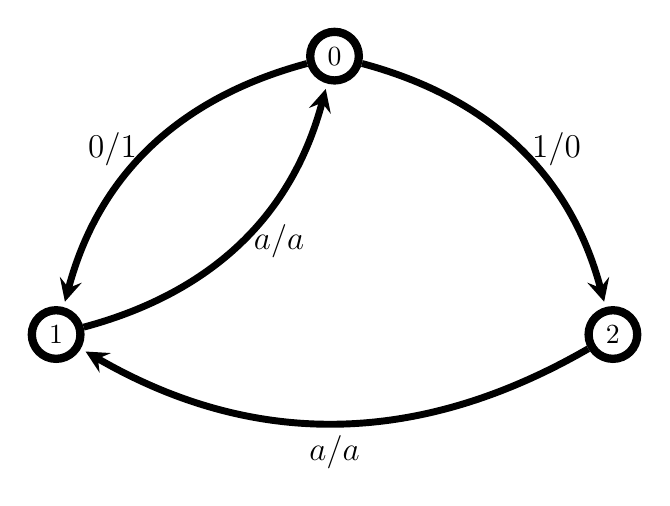
\begin{tikzpicture}[
        ->,
        >=stealth, % arrow head style
        shorten > = 2pt, % don't touch arrow head to node
        node distance=5cm,
        auto]

        \tikzstyle{every state}=[
            draw = black,
            fill = white,
            line width=3pt,
            minimum size = 4mm
        ]
        \tikzstyle{every edge}=[
            draw = black,
            line width=2.5pt,
        ]
        \tikzset{l/.style={font=\large}}
        \node[state] (0) {$0$};
        \node[state] (1) [below left of =0] {$1$};
        \node[state] (2) [below right of =0] {$2$};
        \path
        (0) edge[bend right, left]
        node[l] {$0/1$} (1)
        (0) edge[bend left, right]
        node[l] {$1/0$} (2)
        (1) edge[bend right, right]
        node[l] {$a/a$} (0)
        (2) edge[bend left]
        node[l] {$a/a$} (1)
        ;
    \end{tikzpicture}
\end{center}
For each state $q$ we have length-preserving transduction $\aut{q}$.
These transductions (along with their inverses) form a group
under composition, denoted $\gp{A}$. A transduction $f \in \gp{A}$ is called
\emph{odd} if it flips the first bit of its input; otherwise $f$ is called
\emph{even}. We also have the \emph{residuation} maps $\d{a} :
\gp{\A} \rightarrow \gp{\A}$ for $a \in \{0,1\}$.
In the example above, $\d{0} \aut{0} = \aut{1}$ and
$\d{1} \aut{0} = \aut{2}$.\\

Let $\A$ be a transducer with $n$ states $\{s_1,\ldots,s_n\}$ whose
transduction group is abelian.

\begin{proposition}
    There is an epimorphism $\psi : \Z^n \rightarrow \gp{\A}$ given by
    $\psi\paren{a_1,\ldots,a_n} = \aut{s_1}^{a_1} \cdots \aut{s_n}^{a_n}$
\end{proposition}

\begin{proposition}
    Define the \emph{1/2-transition matrix} as follows:
    \large
    \[
        B_{i,j} = \begin{cases}
            1 & \text{if $\d{0} \aut{s_i} = \d{1} \aut{s_j}$}\\\
            \frac{1}{2} & \text{if $s_i$ is a toggle state and
                $\d{0} \aut{s_i} = \aut{s_j}$ or
                $\d{1} \aut{s_i} = \aut{s_j}$}\\
            0 & \text{otherwise}
        \end{cases}
    \]
    \Large
    Then $B$ performs residuation on even states. That is, for any
    $v \in \Z^m$ such that $\psi(v)$ is even, $\d{a} \psi(v) = \psi (Bv)$.
    \\
\end{proposition}
\end{poster-section}

\begin{poster-section}{Matrix Representations}
\Large
In \cite{nekrashevych2004automorphisms}, Nekrashevych and Sidki proved the
following:
\begin{theorem}
    If $\gp{\A} \cong \Z^m$, then there exists an isomorphism
    $\phi : \gp{\A} \rightarrow \Z^m$, an $m \times m$ matrix $A$, and a
    vector $r$ which satisfy
    \large
    \[
        \phi (\d{a} \aut{p}) = \begin{cases}
            A \cdot \phi(\aut{p}) & \text{if $\aut{p}$ is even}\\
            A \cdot \phi(\aut{p}) + (-1)^a r &
            \text{if $\aut{p}$ is odd}\\
        \end{cases}
    \]
    \Large
    Also, the matrix $A$ satisfies several interesting properties:
    \begin{itemize}
        \item $A$ is contracting, i.e., its spectral radius is less than 1.
        \item The characteristic polynomial $\chi_A(x)$ is irreducible over
            $\Q$, and has the form $\chi_A(x) = x^m + \frac{1}{2}g(x)$ where
            $g(x) \in \Z[x]$ is of degree at most $m-1$.
    \end{itemize}
\end{theorem}
\hfill\\
We call this $A$ and $r$ the \emph{residuation pair} for the automaton
$\A$. We prove some additional properties of $A$.

\begin{lemma}
    The map $R = \psi \circ \phi$ is a surjective linear map
    $\Z^n \rightarrow \Z^m$, and for all $k \ge 1$, $RB^k = A^kR$.
\end{lemma}
\begin{myproof}
    $\psi$ is surjective and $\phi$ is bijective, so $R$ is surjective.
    Since $\psi \circ B = \d{a} \circ \psi$, we have $RB = AR$.
    The claim follows by induction.
\end{myproof}

\begin{lemma}
    The characteristic polynomial of $A$ divides the characteristic
    polynomial of $B$.
\end{lemma}
\begin{myproof}
    By the previous lemma, for any polynomial $P$, $R P(B) = P(A) R$.
    Apply Cayley-Hamilton.
\end{myproof}

\begin{lemma}
    Let $A'$ be the companion matrix of $\chi_A$. We say $A$ is
    well-behaved if $A$ is $GL(m, \Z)$-similar to $A'$, i.e. if
    there exists an invertible $m \times m$ integral matrix $T$ such
    that $TAT^{-1} = A'$. If $A$ is well-behaved, then $(A', Tr)$
    is a residual pair.
\end{lemma}
\begin{myproof}
    For all $v \in \Z^m$ and $c \in \{0, \pm 1\}$,
    \[
        T(Av + cr) = T(T^{-1}A'Tv + cr) = A' (Tv) + c r'
    \]
\end{myproof}

\end{poster-section}

\begin{poster-section}{An Algorithm}
\Large
\begin{theorem}
    There is a polynomial time algorithm to compute a residuation pair
    $A, r$ for a well-behaved abelian automaton $\A$.
\end{theorem}
\begin{myproof}
    For each irreducible factor $f$ of $\chi_B(x)$ of the form
    $x^k + \frac{1}{2}g(x)$ where $g(x) \in \Z[x]$ has degree less
    than $k$, let $C_f$ be the companion matrix of $f$. Solve the matrix
    equation $RB = C_fR$ for $R$, which can be done using Kronecker
    Products. Such a solution is guaranteed to exist because $C_f$
    and $B$ share eigenvalues. Once $R$ is computed, we can compute $r$ as
    follows. Let $s_a$ be an odd state in $\A$ and let $s_b = \d{0} s_a$.
    Let $e_i$ denote the $i$th standard basis vector, such that
    $\psi(e_i) = \aut{s_i}$, and compute $r = Re_b - A'Re_a$.
    We can now simply check if $(C_f, r)$ is a residuation pair for $\A$.
    \\
    By Lemma 2, one of these factors must be $\chi_A$, and since $\A$ is
    well-behaved, $(C_f, r)$ will be a residuation pair for some factor $f$.
\end{myproof}

\begin{theorem}
    The matrix $R$ computed in the above algorithm gives a basis of
    identites holding in $\gp{\A}$.
\end{theorem}
\begin{myproof}
    Since $A'$ is a contraction, $A'^k$ has no nontrivial fixed points for
    all $k > 0$. Thus the only identity in $R(\Z^n)$ is $\vec{0}$, and
    computing the null space of $R$ gives the basis of identites.
\end{myproof}
\end{poster-section}

\begin{poster-section}{References}
    \printbibliography[heading=none]
\end{poster-section}

\begin{poster-section}{Acknowledgements}
    \Large
    Thanks to Klaus Sutner for his guidance on this project. Also, thanks to
    Evan Bergeron for helpful discussions.
\end{poster-section}

\end{multicols}
\end{document}
